\section{Introduction}
\label{intro}
% The very first letter is a 2 line initial drop letter followed
% by the rest of the first word in caps.
% 
% form to use if the first word consists of a single letter:
% \IEEEPARstart{A}{demo} file is ....
% 
% form to use if you need the single drop letter followed by
% normal text (unknown if ever used by the IEEE):
% \IEEEPARstart{A}{}demo file is ....
% 
% Some journals put the first two words in caps:
% \IEEEPARstart{T}{his demo} file is ....
% 
% Here we have the typical use of a "T" for an initial drop letter
% and "HIS" in caps to complete the first word.
\IEEEPARstart{P}{neumonia} is a very common thoracic disease in our life. In clinical practice, a radiologist needs to consider different source of information to decide on the next treatment plan, as a result, multimodal data plays the key role in decision making process. According to the survey, a radiologist of a major hospital need to diagnosis hundreds of pneumonia cases every day. Thus, developing a fast, robust and accurate CAD system to perform automated detection of pneumonia is meaningful and important. 

There have been several methods and epidemiological studies \cite{Franquet2001Imaging}\cite{Thomas2005Standardized}\cite{deepika2018classification} for pneumonia detection and diagnosing, most of them use image data like chest X-ray as their information source.
Hoo-Chang Shin \cite{Shin2016Learning} combined CNN and LSTM \cite{hochreiter1997long}, proposed a model which could describe the contexts of a detected diseases based on the deep CNN features. This model used CNN to extract features from chest X-Ray and used LSTM to generated MeSH \cite{timmurphy.org} terms for chest X-Ray. In 2017, Xiaosong Wang et al. \cite{Wang2017ChestX} provided hospital-scale chest X-ray database ChestX-ray8 which contained eight common thoracic diseases. This database allowed researchers use deeper neural network to analyze thoracic diseases. They tested different pre-trained CNN models on this dataset. Experiments showed that ResNet50 achieved highest AUROC score 0.6333 in classifying pneumonia. They also provided ChestX-ray14 which contains more kinds of thoracic diseases.
Based on this database, later in 2017, Yao et al. \cite{yao2017learning} achieved 0.713 in AUROC score using DenseNet Image Encoder. Pranav Rajpurkar, Andrew Y. Ng et al. \cite{Rajpurkar2017CheXNet} developed CheXnet with 121 convolutional layers and achieved AUROC 0.7680 in pneumonia classification.
In 2018, Xiaosong Wang et al. \cite{Wang2018TieNet} proposed TieNet, which could classify the chest X-Rays into different diseases and generate the report at the same time. In TieNet, CNN was used capture features of chest X-Rays, RNN learned these features and generated report based on attention mechanism, which could help model to focus on different parts of chest X-Ray alone with the generation of reports. In pneumonia classification problem, they achieved 0.947 in AUROC based on report, but they only achieved 0.917 in AUROC on hand-labeled data. 

Studies above have something in common. First of all, they are designed for chest X-Rays. Chest X-rays used to be the best available method for detect pneumonia, played a crucial role in clinical care\cite{Franquet2001Imaging} and epidemiological studies\cite{Thomas2005Standardized}. However, compared to chest X-rays, CT scans have a clearer view of patients' bodies, since bones, skin, vessels, mediastinal and lung tissues may cause overlapping shadows in chest X-ray and cause misdiagnosis. CT allows visualization of lung structures\cite{korfiatis2009texture}, which can help to diagnosis pneumonia in early stage and avoid delayed treatments.
Each slice of CT scans is a 2-D image of human body scan, besides 2-D visual features from CT, you can also reconstruct 3-D structure of human bodies using these slices. Extensive studies show that 3-D CNN is the best choice for keeping 3-D spatial information in CT\cite{Yorozu1987Electron}. However, 3-D CNN cannot be applied to raw CT data directly since it will bring a heavy burden to the server. Radiologists need to accurately measure the lesions, so we cannot reduce the size of images by resizing at will.
 
Second, these models are not designed following the radiologists' diagnosing process but are designed for the convenience of computer vision studies and deep learning model training. For models like CheXnet, image information is the key of models. Few of them combine image visual features with clinical information. Models like TieNet do combine image visual features with descriptions about images written by radiologists. We believe using descriptions about images written by radiologists to improve models is not quite convincing, since descriptions like `Findings' and `impressions' sometimes include diagnosis conclusions.
Patients' chief complaints is a very useful information when doctors are diagnosing \cite{wu2018master}, since chief complaints is patients' direct feeling about their physical condition, telling us the patients' pain location, symptoms and how long have they been ill. Moreover, information of age and gender can provide priori information\cite{xiaojian2011analysis} \cite{huang2014design}. However, as far as we know, few studies use this information to improve CAD systems for pneumonia. 

In general, there are two major drawbacks of existing CAD systems for pneumonia: (1) They cannot handle raw CT scans, which allows visualization of lung structures; (2) Few studies consider clinical information like patients' chief complaints, which is conflict to clinical practice.

To address such drawbacks, we propose a novel Multimodal Data Diagnosis Network(MDDNet) for clinical pneumonia detection. We use raw data collected from The First Affiliated Hospital of Army Medical University, each case contains not only CT image information, but also clinical information about patient gender, age and chief complaint. 

In MDDNet, each CT image will be transformed into a 3-channel image with three windows: Lung Window(LW), High Attenuation(HA) and Low Attenuation(LA). LW provides visual features of normal lung tissues, HA provides visual features of abnormal increase in lung density, LA provides visual features of abnormal decrease in lung density. Three channels complement each other, which not only maintains the ability to extract information from normal lung tissues, but also increases the ability to extract information from abnormal lung tissues.
Besides image data, we also include clinical data in our MDDNet. Chief complaints can provide location of pain, symptoms and how long have patients been ill. These information is related to CT image and enhance the visual features extracted from CT. Moreover, information about age and gender can provide priori information since patients of different age and gender must have differences in the morphology of thoracic cavity and lungs. 
In order to reduce the burden of calculation, we treat CT slices as short video frames and a Recurrent Convolutional Neural Network(RCNN) is used to capture visual features from CT slices. RCNN uses a 2-D CNN to capture visual features from each 2-D slice, and LSTM captures relationships between slices. We use another LSTM to analyze semantics from chief complaints. Information of age and gender will be treated as two extra variables. Our model MDDNet, as shown in Fig~\ref{MMDD}, will learn a joint distribution of all features above and gives out the final classification result.

\begin{figure*}[t]
    \centerline{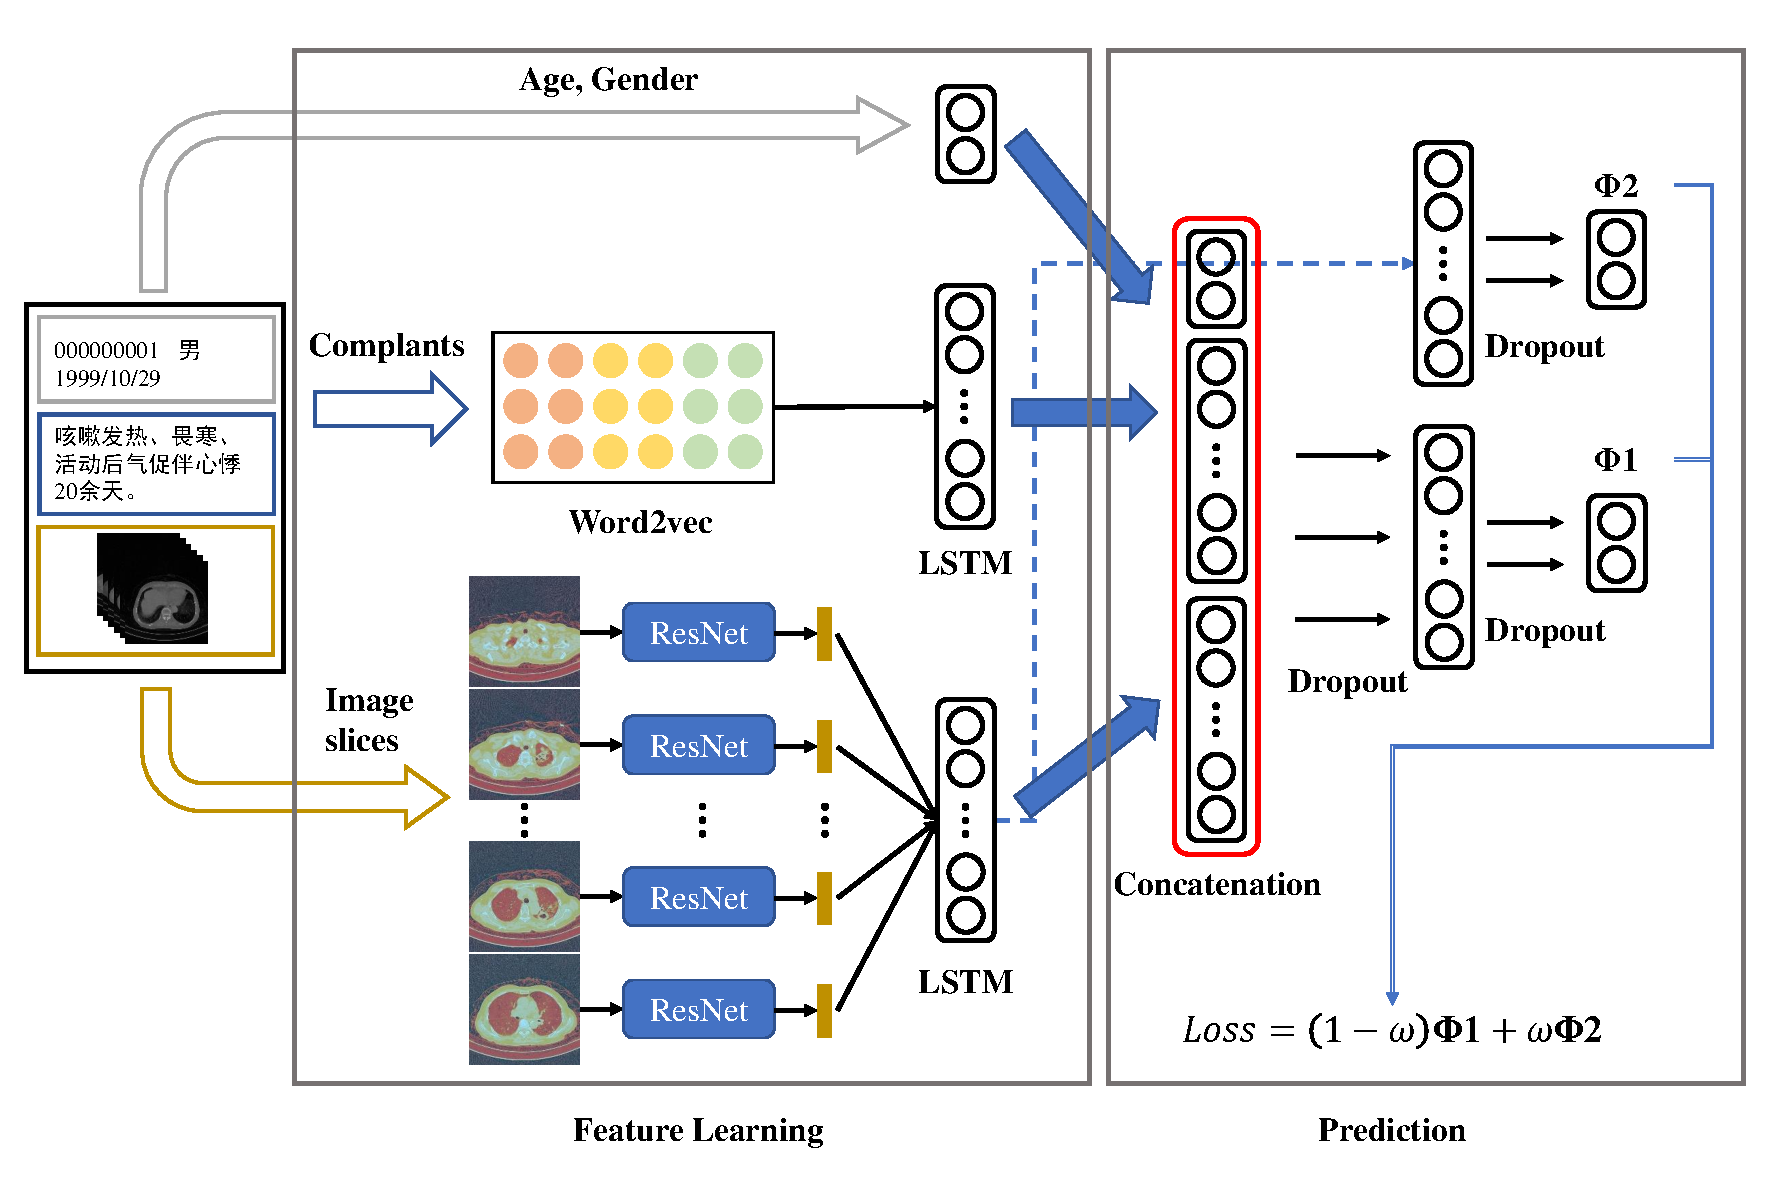
\includegraphics[width=160mm]{MMDD.pdf}}
    \vspace{-0cm}
    \caption{Architecture of MDDNet. The black rectangle contains raw information from hospital. Information in grey rectangle is about age and gender, information in blue rectangle is complaints, information in yellow is CT image data. Chief complaints will be transformed into matrices by Word2vec and analyze by one LSTM network. Image will be fed into RCNN. Age and gender will be treated as two additional features. There three kinds of information will be concatenated in red rectangle and fed into fully-connected layers to get prediction}
    \vspace{-0cm}
    \label{MMDD}
    \end{figure*}


The remainder of the manuscript is organized as follows. 
Section~\ref{methodology} describes the architecture of MDDNet and details of our model.
Section~\ref{experiments} describes the pre-processing steps of dataset and reports our experimental results.
Section~\ref{discuss} further discusses some key points of proposed model and some phenomenons shown during experiments.
Our conclusions are drawn in section~\ref{conclude}.